\section{Limitaciones conocidas de los LLM}
\label{sec:limitaciones_llm}
Ventana de contexto, sesgos, alucinaciones, dar la razón al usuario, 

Seguimos a \cite{arunbijiRAGVsFinetuning}



\subsection{Corte de conocimiento}

Los \gls{llm} no aprenden nuevos datos tras su entrenamiento, por lo que existe una limitación en la información o el conocimiento disponible al no haber tenido acceso a información o acontecimientos ocurridos después de esa fecha límite. Esta limitación se minimiza con rentrenamientos tipo \textit{fine-tuning} o con técnicas como \gls{rag}.

\subsection{Alucinaciones}

La finalidad de un \gls{llm} es <<modelar>> el lenguaje humano, con lo que, a priori, no se puede esperar que los datos que de en sus respuestas sean ciertos sino verosímiles. Los \gls{llm} se entrenan con vastas cantidades de datos de diversa calidad, y la trazabilidad de los datos que devuelve en sus respuestas es muy difícil de determinar. Precisamente, la técnica \gls{rag} permite dibujar la trazabilidad de los datos de las respuestas, en tanto en cuanto estas se basan en los datos de la base de datos de conocimiento. Por otra parte, la constante mejora de los datos de entramiento de los \gls{llm} \citep{gunasekarTextbooksAreAll2023} hace que este problema se minimice aunque nunca se elimina completamente.

\subsection{Ineficiencia y coste}

El tiempo

Memoria RAM

Coste económico


El open source pone su foco en la eficiencia, implementando constantes y rápidas mejoras en la arquitectura de los modelos, su proceso de entrenamiento, la eficiencia en dispositivos de bajos recursos, la creación de conjutos de datos de entreamiento de alta calidad, etc.

El entrenamiento de un \gls{llm} del tamaño de GPT-3\dots

\begin{figure}[H]
  \caption[Coste de entrenamiento en horas de GPU de diversos modelos de lenguaje]{Coste de entrenamiento en horas de GPU de diversos modelos de lenguaje.}
  \centering
  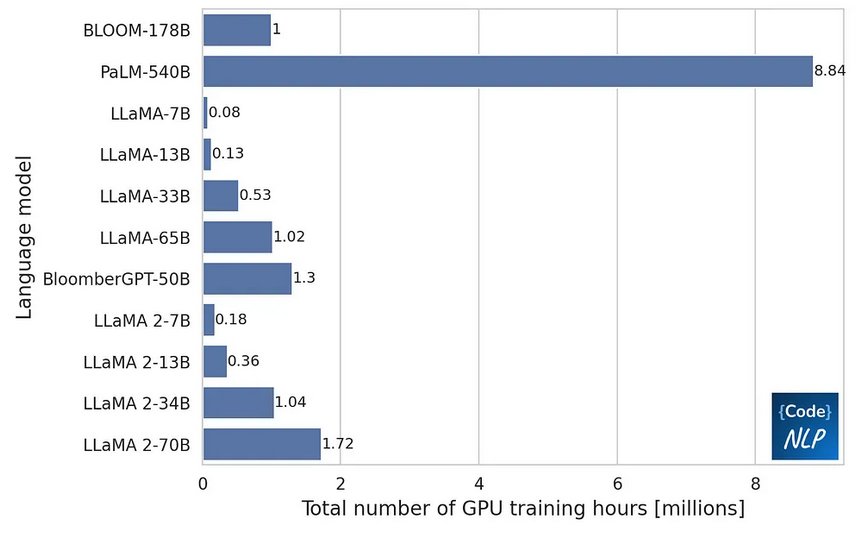
\includegraphics[width=0.8\textwidth]{./figuras/llm_gpu_training_hours.png}
  \source{\cite{ph.dTrainingTimeFoundation2023}}
  \label{fig:llm_gpu_training_hours}
\end{figure}

\subsection{Modelos <<Caja negra>>, sesgos y riesgos}
